% vim: spelllang=fr

\documentclass[../main.tex]{subfiles}
\graphicspath{{\subfix{../Figures/Chap2/}}}
\begin{document}

\begin{itshape}
Ce deuxième chapitre porte de l'approche directe consistant en l'application d'un algorithme de détection et de suivi des cyclones tropicaux dans les modèles
comme façon de caractériser l'activité cyclonique simulée, ainsi que la façon dont les modèles représentent ces phénomènes. Un cas d'étude est présenté via
l'application du schéma de détection du CNRM à la réanalyse ERA5.
\end{itshape}

\minitoc\newpage
%--------------------------------------

\section{Introduction}\label{sec:intro_chap2}

Les algorithmes de détection et de suivi des HTV dans les modèles consistent à identifier les points de grille qui satisfont des critères thermiques ou
dynamiques associés à un cyclone tropical. Le \cref{chap:chapitre_1}, en particulier la \cref{sec:intro_tracking}, met en évidence la sensibilité de l'activité
cyclonique mesurée au choix de la méthode de détection et montre que ce choix peut aboutir à des conclusions différentes quant au signe du changement dans des
expériences à climat plus chaud. En effet, si tous les traqueurs de TC partagent le même objectif, les méthodologies utilisées dans la littérature présentent
néanmoins une très grande diversité. Les premiers schémas de détection étaient basés uniquement sur la MSLP et la vitesse des vents
\parencite{bengtsson_simulation_1982,broccoli_can_1990}, tandis que \cite{haarsma_tropical_1993,bengtsson_hurricanetype_1995} ajoutèrent à cela des critères sur
la vorticité ainsi qu'un diagnostique sur la présence d'un cœur chaud, dans l'optique de discriminer les perturbations tropicales de leurs homologues
extra-tropicales. \cite{wu_gcm_1992} utilisèrent des critères supplémentaires conçus pour discriminer les perturbations tropicales sèches via un seuil
d'humidité relative, les perturbations équatoriales d'est en interdisant le vent d'est à \hPa{950} au point situé à \ang{4.5} au nord et au sud du cyclone,
ainsi que les perturbations barocliniques en bornant la vitesse du vent d'ouest à \hPa{200} au dessus du centre du cyclone à \ms{5}. Dans
\cite{bengtsson_hurricanetype_1995}, la méthodologie de détection introduit des tests de structure verticale du système, aussi bien sur le profil de vent que de
température. En effet, après avoir identifié un centre cyclonique à travers la vorticité, pression minimum locale et vitesse du vent maximale dans une boîte
autour du système, il s'agit alors de s'assurer de la présence d'une anomalie de température sur l'ensemble de la troposphère, par rapport à la moyenne prise
dans cette boîte, puis de s'assurer également que l'anomalie à la tropopause est supérieure que celle à la couche limite. Un test similaire est réalisé sur le
profil vertical de vent, en imposant que le vent moyen à \hPa{850} supérieur à la moyenne du niveau à \hPa{300}, toujours dans la boîte centrée. Beaucoup
d'algorithmes de détection reprennent cette méthodologie, avec quelques variantes et spécificités. Une grande quantité de méthodologies et de seuils de
détection sont décrits dans \cite{walsh_objectively_2007} ainsi que dans \cite[][Annexe B]{ullrich_tempestextremes_2017}, schémas dans lesquels la définition
d'un TC et les valeurs numériques utilisées pour les divers seuils de détection sont souvent choisis de telle sorte à reproduire au mieux la climatologie
observée \parencite{walsh_objectively_2007,tory_development_2013}.

Parmi les traqueurs possédant des particularités remarquables, le plus communément utilisé est sans aucun doute le schéma de détection TRACK
\parencite{hodges_how_2017}. Ce dernier a la particularité de systématiquement interpoler les champs du modèle à une basse résolution (T63, soit \km{210}),
avant d'appliquer un schéma de détection basé exclusivement sur la vorticité. Cela permettrait de s'affranchir de la sensibilité de la méthode de détection à la
résolution du modèle. Cet algorithme a cependant tendance à détecter une quantité parfois anormalement élevée de systèmes (voir \cref{fig:NTC_HighResMIP_TRACK}
par rapport à la \cref{fig:NTC_HighResMIP}), et est alors particulièrement sujet à la détection de faux-positifs \parencite{bourdin_intercomparison_2022}. La
problématique que TRACK vise à solutionner est néanmoins bien réelle. La résolution du modèle impacte la représentation des TC dans les modèles ce qui implique
que les traqueurs doivent souvent être ajustés pour chaque résolution. Une autre alternative se trouve dans \cite{camargo_improving_2002} où les auteurs ont
proposé une méthode de détection de HTV dont les seuils pour chacune des variables sont déterminées à partir de la climatologie du modèle. Spécifiquement, ces
derniers s'expriment sous la forme $\alpha \sigma + \beta$, où $\alpha$ et $\beta$ sont issues de la climatologie globale du modèle, et où $\sigma$ représente
l'écart type de la variable à l'échelle de chaque bassin océanique. La méthode de \cite{camargo_improving_2002} n'est cependant pas largement répandue,
possiblement parce que d'une part, les valeurs $\alpha$ et $\beta$ pour chacune des variables se déterminent par les densités de probabilités bivariées dont
l'estimation est complexe et laborieuse, et d'autre part parce que cette approche représente un paradigme très différent des traqueurs mentionnés précédemment.
En effet, les traqueurs à seuils fixes visent à appliquer un schéma de fonctionnement conceptuel d'un cyclone tropical au modèle, ce qui permet ensuite
d'établir dans quelle mesure le modèle est capable de simuler des systèmes réalistes, là où la méthode de \cite{camargo_improving_2002} cherche au contraire à
s'affranchir des biais intrinsèques au modèle, en considérant que les TC constituent dans tous les cas les extrêmes des distribution des variables d'intérêt. Il
faut cependant noter que si les traqueurs à seuils absolus permettent d'évaluer des biais de représentation des TC, ils ont également le défaut de rendre
indiscernables les erreurs issues du modèle de celles issues du schéma de détection lui-même, contribuant aux incertitudes quant à l'évolution future de la
fréquence des cyclones tropicaux dans un climat plus chaud mentionnées dans le \cref{chap:chapitre_1}, \cref{sec:intro_tracking}. Ces deux catégories de
traqueurs ont donc chacun leurs avantages et leurs inconvénients.

Ainsi, pour espérer comprendre la divergence entre les projections issues de l'approche directe et indirecte, il est nécessaire de pouvoir évaluer
quantitativement la performance d'un schéma de détection et de suivi objectif de cyclones tropicaux. Une solution consiste à appliquer un schéma de détection à
une simulation dont les trajectoires sont à priori connues d'avance, en utilisant une réanalyse atmosphérique. Les réanalyses combinent des prévisions
météorologiques à court terme avec des observations passées via un modèle et un schéma d'assimilation de données ---~permettant de corriger la trajectoire du
modèle lorsque ce dernier s'éloigne de l'état connu de l'atmosphère~--- invariants sur toute la période d'analyse. Une réanalyse offre donc une vision globale
de l'atmosphère qui est cohérente dans le temps et l'espace et qui intègre au mieux l'ensemble des observations qui y sont intégrées, si bien que le produit
final constitue une excellente estimation de l'état passé de l'atmosphère sur toute la période considérée. Il en résulte que la plupart ---~sinon
l'intégralité~--- des cyclones tropicaux observés et référencés dans la base données IBTrACS, introduite dans le \cref{chap:chapitre_1},
\cref{sec:observations}, sont à priori présents dans une réanalyse.

Dans ce chapitre, on considère le schéma de détection du CNRM, à l'origine conçu pour suivre les dépressions de moyennes latitudes par
\cite{ayrault_nouvelle_2000} puis adapté aux cyclones tropicaux dans \cite{chauvin_response_2006}, et utilisé à cette fin par
\cite{daloz_impact_2012,chauvin_atlantic_2017,chauvin_future_2020,cattiaux_projected_2020}. Des descriptions détaillées du fonctionnement de cet algorithme sont
disponibles dans \cite{chauvin_response_2006}, ainsi que dans la \cref{sec:papier_data_methods}. Spécifiquement, le traqueur du CNRM est appliqué à la réanalyse
ERA5 \parencite{hersbach_era5_2020}. En effet, ERA5 est la dernière en date du CEPMMT et est la première réanalyse mondiale à atteindre une résolution
horizontale de \km{31}, ici interpolée sur une grille à \ang{0.25}. Elle assimile des données issues de plus d'une vingtaine de satellites d'observations
météorologiques, totalisant \num{54} instruments. Aux données satellitaires s'ajoutent les observations \textit{in-situ} composées de stations au sol, bouées
instrumentées, navires marins, radiosondages, radars et avions de reconnaissance. De par sa résolution inédite et la grande diversité des sources observations
qui y sont assimilées, ERA5 constitue donc le choix idéal pour évaluer la capacité du traqueur à détecter les HTV. Dans la \cref{sec:eval_tracker_ERA5}, les
performances du traqueur du CNRM ainsi que sa sensibilité à ses divers seuils de détection sont évaluées sur ERA5, en termes de probabilité de détection
(\textit{Probability of Detection}, POD) et de taux de fausses alarmes (\textit{False Alarm Rate}, FAR). La capacité d'ERA5 à représenter les TC est également
évaluée, via une analyse de leurs caractéristiques en termes d'intensité, de cycle de vie et également via l'étude de leur profiles verticaux. Ces travaux sont
présentés par la publication scientifique dont ils ont fait l'objet \parencite{dulac_assessing_2023}. Un article complémentaire compare les tracks issues de
quatre schémas de détection appliqués à ERA5, dont celui du CNRM \parencite{bourdin_intercomparison_2022}. Enfin, la \cref{sec:complements_papier} présente des
considérations sur le filtrage de systèmes de moyennes latitudes ---~source de biais important dans les schémas de détection de TC---~ ainsi qu'une possible
alternative au FAR et au POD comme métrique d'optimisation, via l'évaluation de la similarité des trajectoires détectées dans ERA5 par rapport aux trajectoires
historiques.

\section{Évaluation du traqueur CNRM sur ERA5 par rapport à IBTrACS}\label{sec:eval_tracker_ERA5}

\subsection{Résumé de l'article}

La réanalyse ERA5 du Centre européen pour les prévisions météorologiques à moyen terme est la première réanalyse mondiale à atteindre une résolution horizontale
de \km{31} et offre donc une occasion unique d'étudier les cyclones tropicaux, et en particulier les champs 3D associés aux TC historiques. A cette fin, un
algorithme de détection et de suivi des TC spécialement calibré pour ce jeu de données est appliqué sur ERA5 ainsi qu'un algorithme d'appariement des
trajectoires conçu pour associer les trajectoires détectées avec celles issues de la base de données IBTrACS dans le but d'évaluer la capacité de la réanalyse à
représenter les cyclones tropicaux Après optimisation du schéma de suivi et l'application d'une technique de filtrage dynamique des systèmes de moyennes
latitudes, il est montré que la majorité des TC d'IBTrACS sont détectés dans ERA5 et que le nombre de fausses alarmes reste raisonnablement bas dans la plupart
des régions. En comparant les trajectoires détectées dans ERA5 avec leurs équivalents IBTrACS, on constate que l'intensité des TC est encore fortement
sous-estimée dans la réanalyse, mais que la distribution de la pression minimale au niveau de la mer est mieux représentée que la vitesse maximale du vent. Par
ailleurs, la comparaison entre les cycles de vie des deux jeux de données met en évidence des différences essentielles entre ERA5 et les best tracks, avec en
particulier un retard avec lequel les TC d'ERA5 atteignent leur pic d'intensité par rapport à IBTrACS, délai qui augmente de manière significative pour les
cyclones les plus forts. Enfin, les structures verticales des TC dans la réanalyse sont analysées et révèlent une intensification nette jusqu'à la catégorie 3
sur l'échelle de Saffir-Simpson, au delà de quoi les différences sont peu discernables.

La version publiée de \cite{dulac_assessing_2023} est présentée dans la \cref{sec:papier} ci-après, avec la permission de l'éditeur \textit{Springer Nature}.

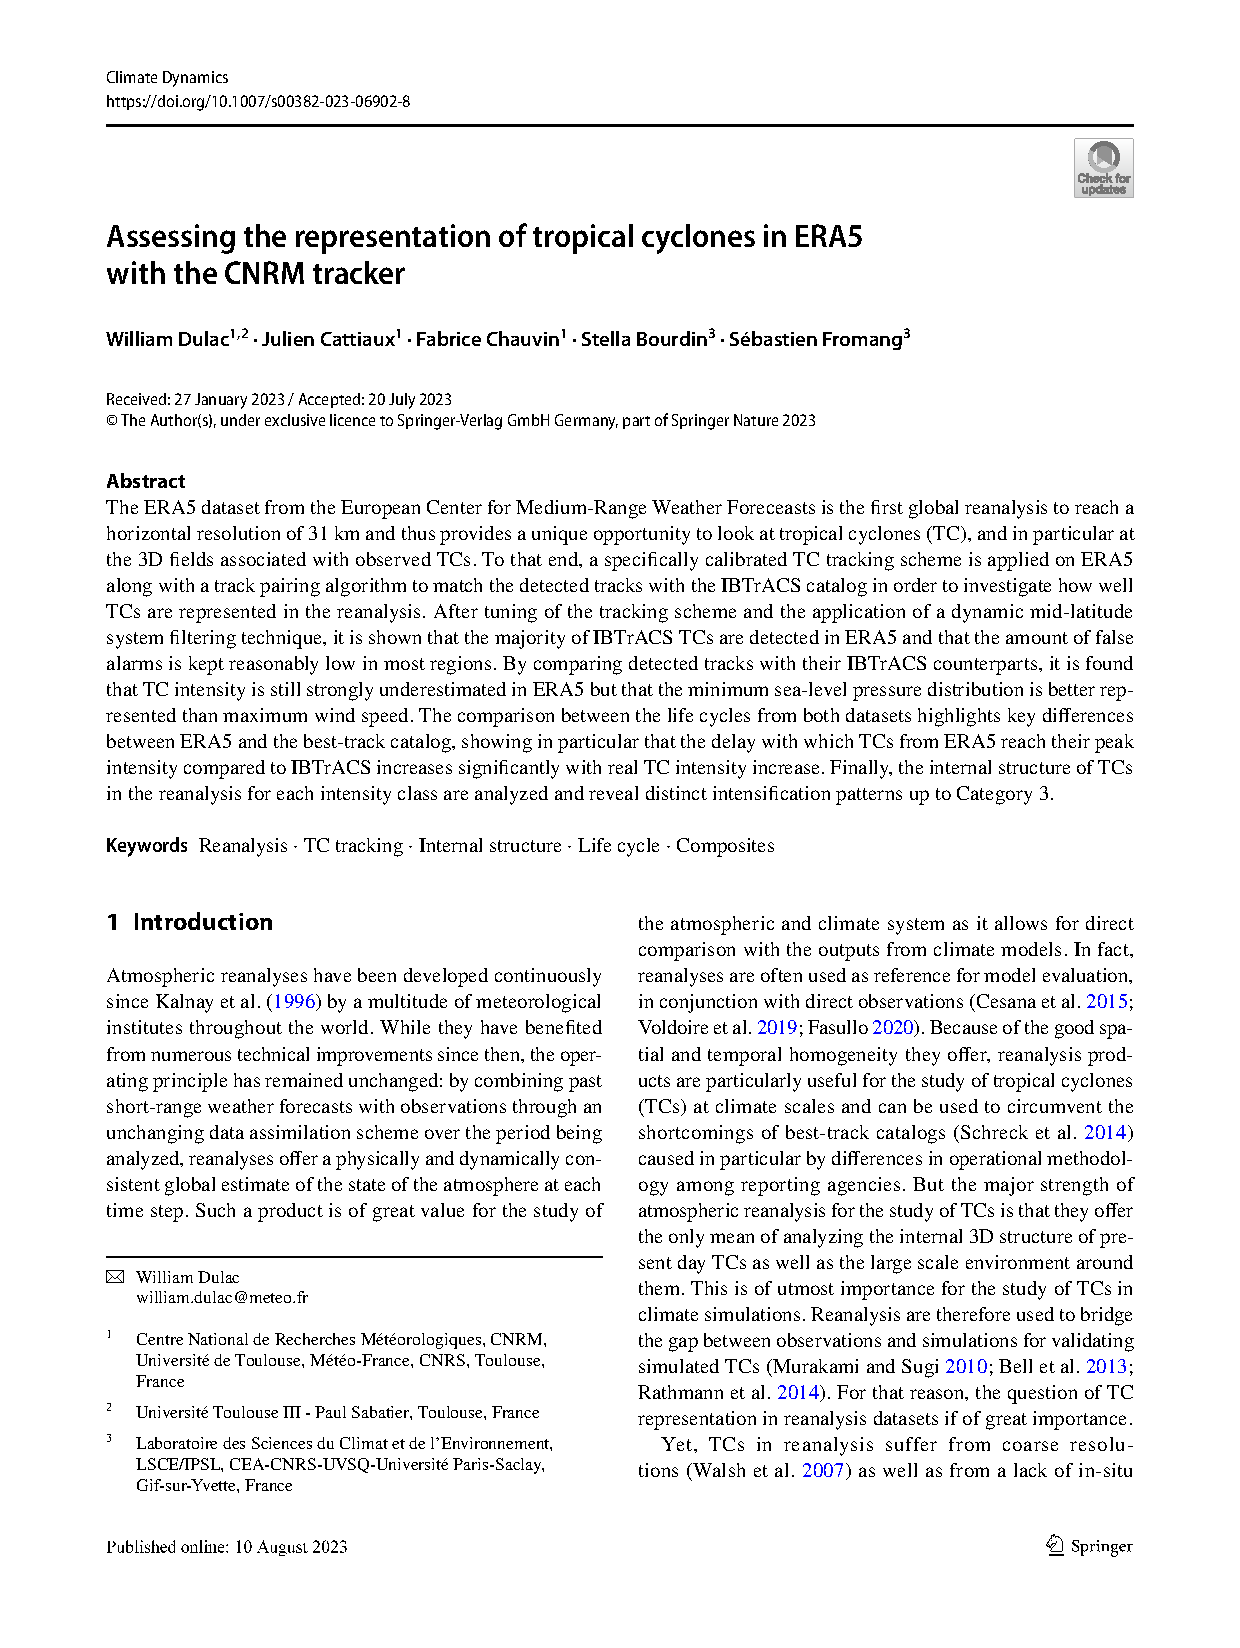
\includepdf[pages=-,pagecommand={\thispagestyle{plain}},offset=5mm 0mm,scale=1,addtotoc=
    {1,subsection,1,Article Climate Dynamics,sec:papier,
     1,subsubsection,2,Introduction,sec:papier_intro,
     2,subsubsection,2,Données et Méthodes,sec:papier_data_methods,
     4,subsubsection,2,Résultats,sec:papier_results,
     10,subsubsection,2,Discussion et conclusion,sec:papier:discussion,
     12,subsubsection,2,Annexe A: Optimisation du traqueur pour ERA5,sec:papier_appendix_A}]{\subfix{../include/dulac2023.pdf}}
%
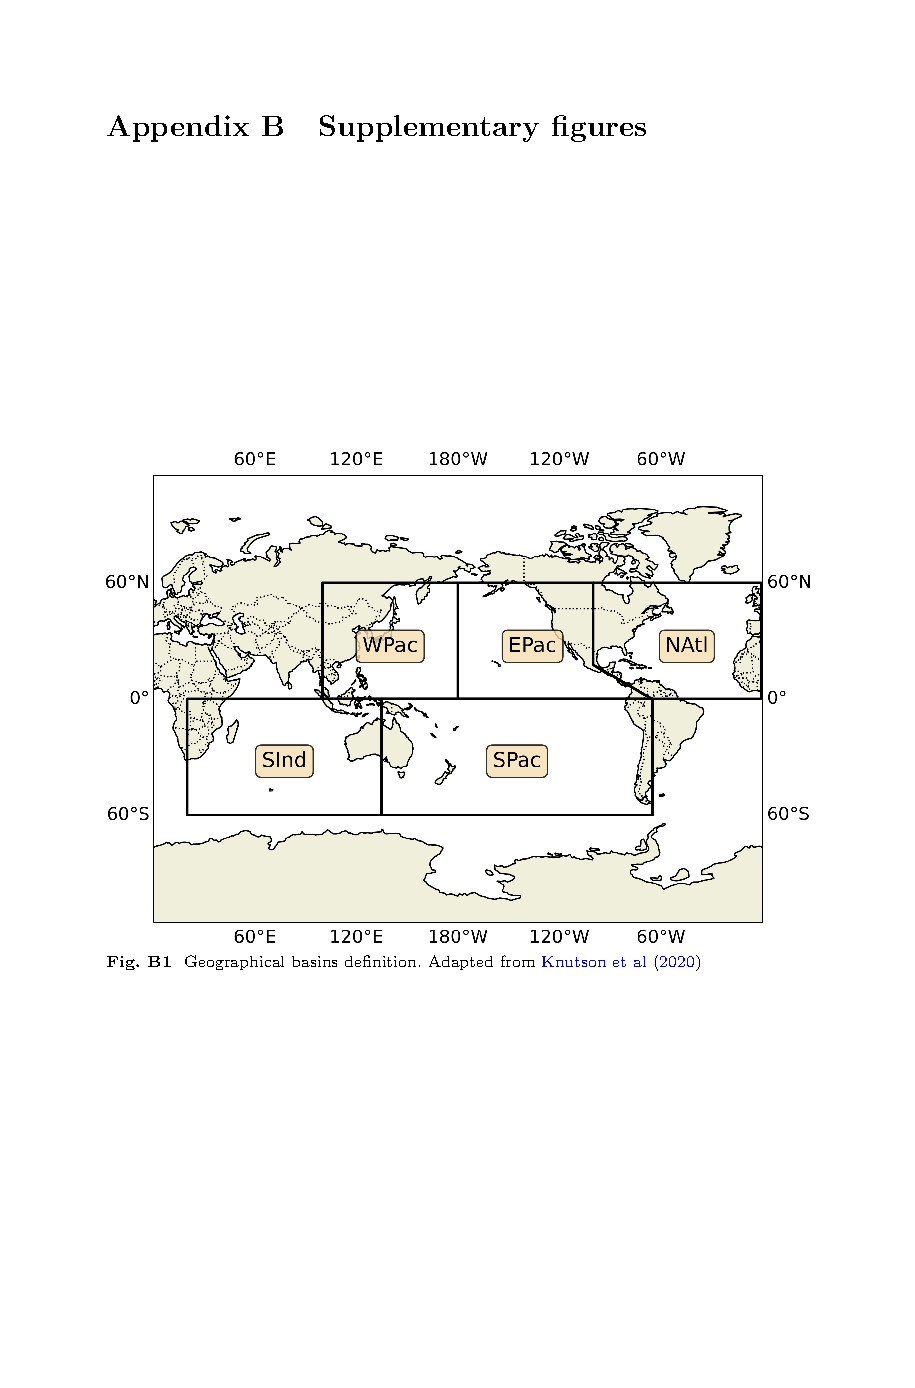
\includepdf[pages=-,pagecommand={\thispagestyle{plain}},offset=5mm 0mm,addtotoc=
{1,subsubsection,2,Annexe B: Figures supplémentaires,sec:papier_appendix_B}]{\subfix{../include/appendix_B_empty.pdf}}

\section{Compléments}\label{sec:complements_papier}

\subsection{Filtrage des systèmes de moyennes latitudes}\label{sec:filtrage_mid_latitudes}

\subsection{Métriques d'évaluation de la similarité des trajectoires}\label{sec:similarité}

\subsubsection*{Introduction}

Les travaux réalisés dans \cite{dulac_assessing_2023} et présentés dans la \cref{sec:papier} font appel aux notions de FAR et POD pour évaluer la performance de
le schéma de détection de TC du CNRM. Le calcul du POD s'appuie sur un algorithme qui associe les trajectoires détectées dans ERA5 à celles présentes dans la
base de données IBTrACS par correspondance spatio-temporelle. Si en moyenne le taux de recouvrement des trajectoires appariés (\textquote{\textit{matched}} dans
\cite{dulac_assessing_2023}) ---~c'est à dire le nombre de points ERA5 situés à moins de \km{300} d'IBTrACS rapporté au nombre d'échéances de la trajectoire
IBTrACS, tel que défini dans la \cref{sec:papier_data_methods}~--- est de \prct{68} (médiane à \prct{71}), il suffit dans l'absolu d'un seul pas de temps
remplissant la condition pour que la trajectoire ERA5 soit appariée à une trajectoire présente dans les observations, et donc pour que la trajectoire détectée
contribue au POD. Ce cas est néanmoins rare puisqu'il concerne en tout et pour tout \num{7} paires de trajectoires ERA5 / IBTrACS, mais on note cependant que
près de \prct{4} de nos trajectoires ERA5 ont un taux de recouvrement inférieur ou égal à \prct{25}. Par ailleurs, le taux de recouvrement des couples de
trajectoires ainsi formés tend à augmenter avec l'intensité des cyclones observés, comme le montre la \cref{fig:coverage_ratio} encadré (a), et qui s'explique
par le fait que les cyclones les plus intenses sont les plus facilement détectables par le traqueur. Cette tendance à de meilleurs recouvrements pour les
cyclones les plus forts n'empêchent pas une certaine dispersion des valeurs. Par exemple \prct{5} des trajectoires appariés à des TC de catégorie \num{3} ont un
taux de recouvrement inférieur ou égal à \prct{31}. Une partie de la variance dans ces scores peut s'expliquer par le fait que le traqueur du CNRM est
susceptible de manquer le début et la fin du cycle de vie des trajectoires observées, en dépit du mécanisme de relaxation des paramètres utilisé dans le schéma
de détection \parencite[][Figure 8]{bourdin_intercomparison_2022}, auquel cas le recouvrement s'en voit mécaniquement réduit. L'autre facteur est que les
trajectoires ERA5 peuvent localement s'éloigner à plus de \km{300} d'IBTrACS. La \cref{fig:coverage_ratio} encadré (b) montre la distribution de la fraction des
points ERA5 situés à plus de \km{300} des observations pour chaque paire de trajectoire et montre qu'en moyenne \prct{5.8} des points détectés par le traqueur
parmi les trajectoires appariés à IBTrACS sont au delà de la limite d'appariement. De plus, \prct{5} des trajectoires détectées dans ERA5 ont une fraction
divergente d'au moins \prct{26}. Par conséquent, la trajectoire détectée dans la réanalyse n'est pas toujours identique à celle du catalogue des best tracks,
soit parce que le traqueur n'en détecte qu'une partie, soit parce que la trajectoire détectée diverge des observations, ou encore par une combinaison quelconque
de ces deux éléments. Enfin, bien que le taux de recouvrement donne une indication sur la similarité des deux trajectoires, il n'apporte pas d'information sur
les variations locales dans la direction de déplacement, si bien que ce dernier n'est pas adapté pour évaluer quantitativement la ressemblance entre les
trajectoires détectées dans la réanalyse et celles issues des observations.

\begin{figure}[tb]
    \centering
    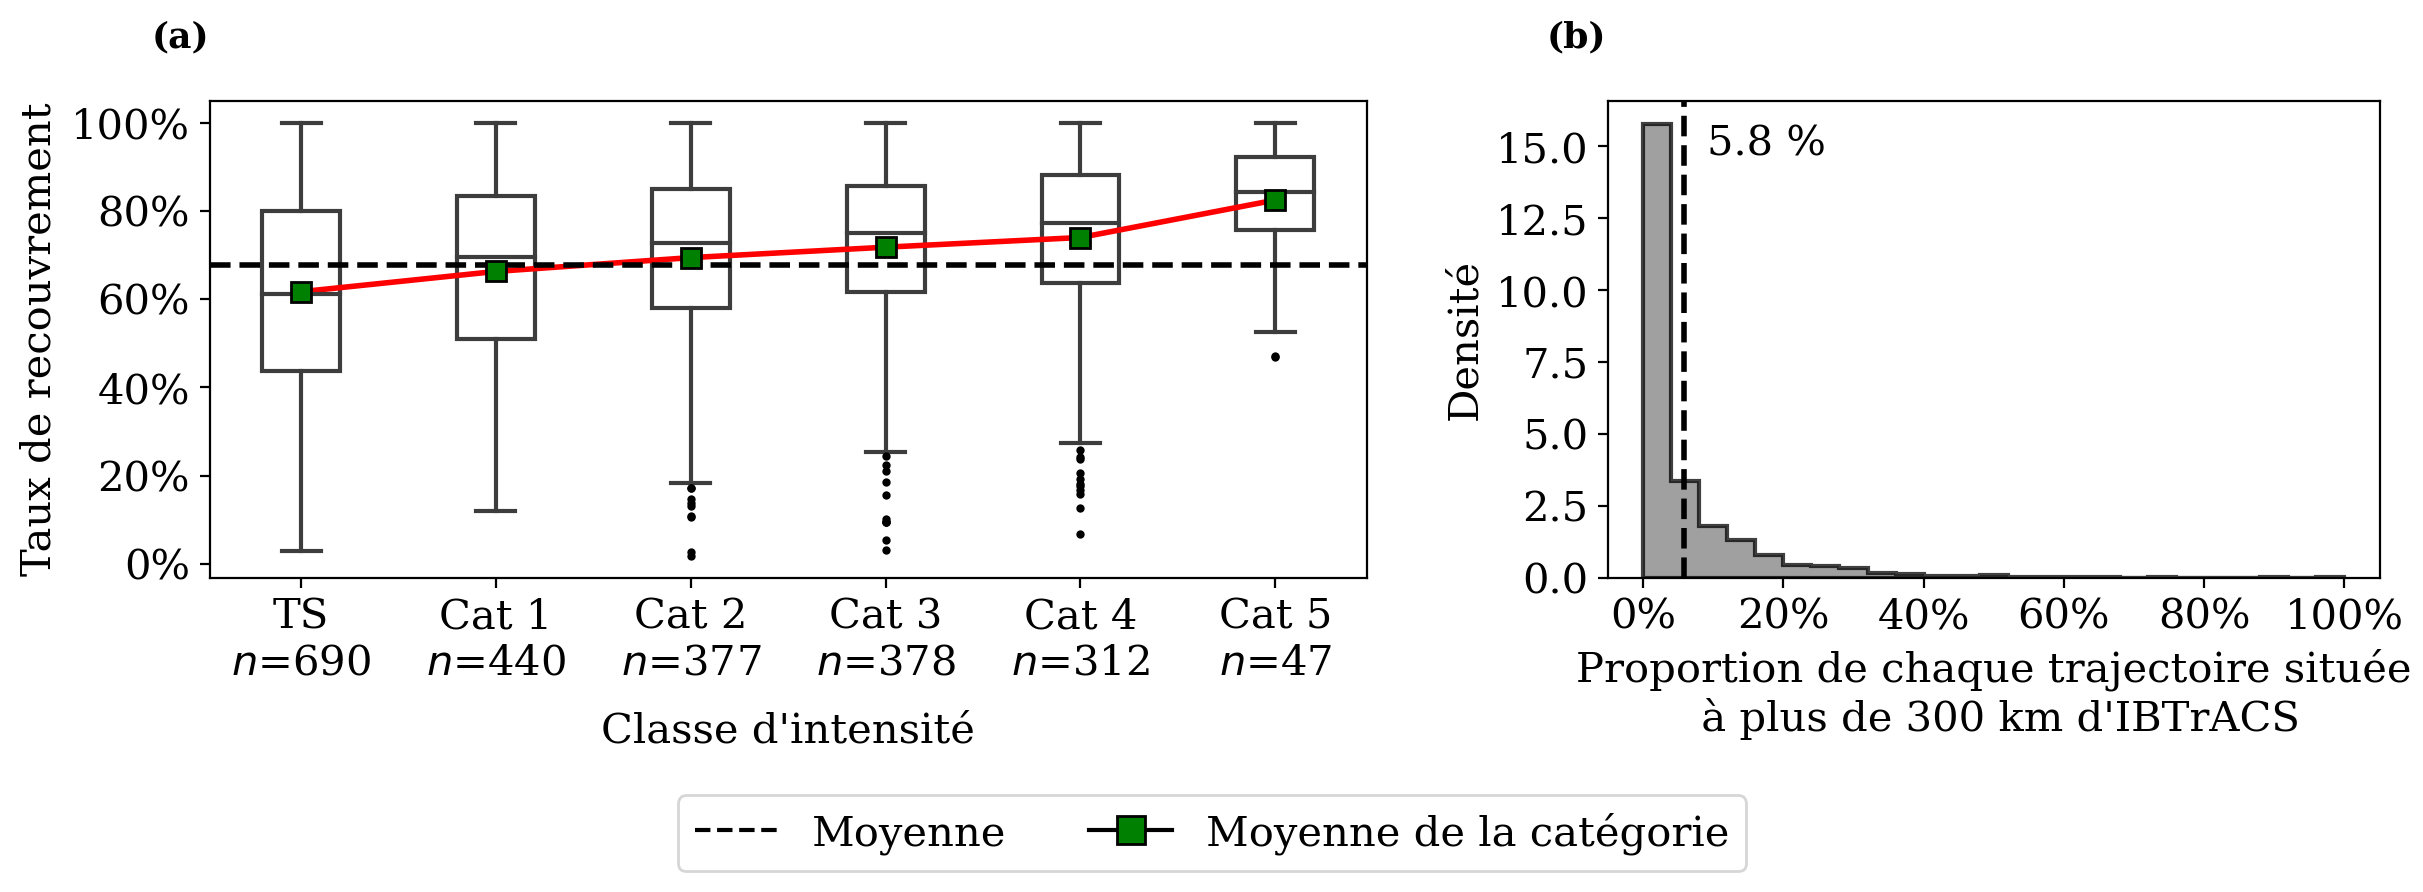
\includegraphics[width=\textwidth]{coverage_ratio_and_missed.png}
    \caption{\textbf{(a)} Distributions des taux de recouvrement des trajectoires appariées entre ERA5 / IBTrACS pour chaque classe d'intensité des TC observés.
    \textbf{(b)} Histogramme de la fraction de points détectés situés à plus de \km{300} d'IBTrACS parmi les trajectoires appariés.}
    \label{fig:coverage_ratio}
\end{figure}

Il existe dans la littérature des algorithmes d'évaluation de la similarité de séries temporelles
\parencite{faloutsos_fast_1994,das_finding_1997,frentzos_indexbased_2007}, mais ces derniers sont plutôt conçus pour des séries uni-dimensionnelles que pour des
trajectoires spatiales car sont souvent basés sur la distance euclidienne qui les sépare. \cite{nakamura_shapebased_2013} proposent une approche basée plutôt
sur la mesure de la similarité de la forme entre deux séries par l'analyse de l'angle formé par les séries, métrique nommée \textit{Angular Metric for Shape
Similarity} (AMSS). Bien que leur approche soit pleinement capable de s'appliquer à des trajectoires spatiales, certaines propriétés de leur métrique ne sont
pas pertinentes (voire pas souhaitables), dans le cas précis des trajectoires de cyclones tropicaux, telles qu'une forte résilience à un décalage temporel entre
les deux séries (pas applicable à des trajectoires appariées entre réanalyse et observations), ainsi qu'une robustesse à des changements isolés de direction.
Ces propriétés rendent par ailleurs leur algorithme très couteux en temps de calcul. Néanmoins, l'aspect novateur derrière les travaux de
\cite{nakamura_shapebased_2013} est repris ici, à savoir la décomposition de la trajectoire en série de vecteurs, détaillée ci-après. Dans cette section, trois
métriques de similarité des trajectoires sont définies et comparées sur le jeu de données issu de \cite{dulac_assessing_2023} et composé des trajectoires
détectées dans la réanalyse ERA5 qui sont appariées à des trajectoires historiques IBTrACS. En particulier, cette analyse vise à déterminer si le réglage des
seuils de détection du traqueur de TC du CNRM dans le but de maximiser le POD ne risque pas de produire des trajectoires peu ressemblantes, du fait de la
formulation de la condition nécessaire et suffisante à l'appariement de deux trajectoires. Leur utilisation comme possible métrique d'optimisation d'un schéma
de détection est discutée.

\subsubsection*{La similarité angulaire}

Une trajectoire de cyclone tropical est une série temporelle composée des positions successives du système et accompagnées de diverses informations permettant
la caractérisation du système, telles que le vent maximum ou la pression centrale. Pour pouvoir évaluer la similarité entre deux trajectoires, on considère non
pas les positions discrètes du système, mais plutôt la série de vecteurs décrivant le déplacement relatif entre chaque position successive.

Reprenant le formalise de \cite{nakamura_shapebased_2013} ; soit $C$ une trajectoire de TC composée de $M+1$ pas de temps et définie par ses positions
$p_{1...M+1}$ sur une grille géo-référencée et aux temps $t_{1...M+1}$ :
%
\begin{align*}
    C &= ((p_1, t_1), (p_2, t_2), \ldots, (p_{M+1}, t_{M+1}))\\
      &= (c_1, c_2, \ldots, c_{M+1})
\end{align*}
%
Alors la série des vecteurs de déplacement équivalente $C_{\text{vec}}$ est donnée par :
\begin{align*}
    C_{vec} &= ((c_2 - c_1), (c_3 - c_2), \ldots, (c_{M+1} - c_M))\\
            &= (\vec{c_1}, \vec{c_2}, \ldots, \vec{c_M})
\end{align*}
%
Soit $Q_{\text{vec}}$ la série des vecteurs de déplacements d'une seconde trajectoire composée de $N$ vecteurs. On définit la similarité cosinus $S_C$ entre
deux des vecteurs individuels $\vec{c}_i$ et $\vec{q}_j$ issus respectivement de $C_{\text{vec}}$ et $Q_{\text{vec}}$, et où $i$ et $j$ correspondent au même
temps $t$ par :
%
\begin{equation*}
    S_C(\vec{c}_i, \vec{q}_j) = \cos \theta = \frac{\vec{c}_i \cdot \vec{q}_j}{\lVert \vec{c}_i \rVert \lVert \vec{q}_j \rVert} \in [-1; 1] 
\end{equation*}
%
Ainsi la similarité cosinus caractérise l'angle formé par les vecteurs de déplacement issus de deux trajectoires à un instant donné. On peut ensuite définir la
distance angulaire, ou angle normalisé, qui est une distance formelle au sens où l'inégalité de Cauchy-Schwartz est respectée, par :
%
\begin{equation*}
    D_\theta = \frac{\theta}{\pi}
\end{equation*}
%
Et son complément, appelé similarité angulaire par :
%
\begin{equation*}
    S_\theta = 1 - D_\theta = 1 - \frac{\theta}{\pi} \in [0; 1]
\end{equation*}
%
C'est cette dernière distance $S_\theta$ qui est utilisée dans cette analyse. De cette façon, la plus faible similarité entre deux vecteurs est atteinte
lorsqu'ils sont parallèles mais de sens opposés, tandis que la similarité est maximale si deux vecteurs parallèles sont de même sens.

\subsubsection*{Métriques de similarité intégrée}

Avant de détailler les trois métriques, il est important de distinguer trois membres dans un couple de trajectoires appariées. En effet, la similarité angulaire
$S_\theta$ est définie ci-dessus pour deux vecteurs correspondants aux déplacements entre deux positions successives, pour deux trajectoires prises au même
temps $t$. Or, il est admis qu'un des deux vecteurs peut ne pas exister à cet instant si le schéma de détection n'a pas capturé l'entièreté de la trajectoire
ou au contraire si la trajectoire détectée est plus longue que celle observée. On appelle donc l'intersection des trajectoires $C \cap Q$ le sous-ensemble des
pas de temps dans lequel les deux trajectoires co-existent. Réciproquement, l'union $C \cup Q$ contient l'ensemble des échéances des deux trajectoires. Enfin,
la différence symétrique des deux trajectoires $C \ominus Q$ contient les pas de temps pour lesquels une seule trajectoire existe à la fois.


%--------------------------------------
\section{Synthèse}

\end{document}
